%%%%%%%%%%%%%%%%%%%%%%%%%%%%%%%%%%%%%%%
% Deedy CV/Resume
%
% Original author:
% Debarghya Das (http://www.debarghyadas.com)
% With extensive modifications by:
% Vel (vel@latextemplates.com)
%
% License:
% CC BY-NC-SA 3.0 (http://creativecommons.org/licenses/by-nc-sa/3.0/)
%
% Important notes:
% This template needs to be compiled with XeLaTeX.
%
%%%%%%%%%%%%%%%%%%%%%%%%%%%%%%%%%%%%%%

\documentclass[letterpaper]{my-resume} 

\usepackage{graphicx} % Picture
\usepackage[absolute]{textpos} % Picture + QRCode
\usepackage{verbatim} % Multiline comments 

%\begin{comment}
%\end{comment}

\begin{document}

\begin{textblock}{2.5}(5,2)
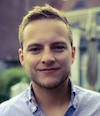
\includegraphics[scale=0.75]{profil.jpg}
\end{textblock}

\begin{textblock}{2.5}(78,4)

\includegraphics[scale=0.30]{qrcode.png}
\end{textblock}

%----------------------------------------------------------------------------------------
%	HEADER SECTION
%----------------------------------------------------------------------------------------

\lastupdated % Print the Last Updated text at the top right

\namesection{Maxime}{Hardy}{
\urlstyle{same}\url{http://hardy.im} \\
\textbf{Front-End Web Developer} \\
\href{mailto:maxime@hardy.lu}{maxime@hardy.lu} | (+44) 07783 126066 \\
}

%----------------------------------------------------------------------------------------
%	LEFT COLUMN
%----------------------------------------------------------------------------------------

\begin{minipage}[t]{0.33\textwidth}

%------------------------------------------------
%	EDUCATION
%------------------------------------------------

\section{Education} 

\subsection{Stafford House School}

\location{Expected Apr 2016 | London, UK}

\descript{Business English and general English lessons}

\sectionspace

%------------------------------------------------

\subsection{Paul Lambin Institute}

\location{Expected June 2015 | Brussels, BE \\ Cum. GPA: 71,83\%}

\descript{BSc with Distinction in information technology}

\sectionspace

%------------------------------------------------

\subsection{Uni. libre de Bruxelles}

\location{2010 - 2012 | Brussels, BE \\ Cum. GPA: N/A}

\descript{Preparatory training in computer science}

\sectionspace

%------------------------------------------------

\subsection{Saint-Louis Institute}

\location{Expected Dec 2010 | Brussels, BE \\ Cum. GPA: N/A}

\descript{Mathematics courses}

\sectionspace

%------------------------------------------------
%	LINKS
%------------------------------------------------

\section{Links} 

LinkedIn:// \href{https://www.linkedin.com/in/maximehardy}{\bf maximehardy} \\
GitHub:// \href{https://github.com/mxhuk}{\bf mxhduk} \\
Twitter:// \href{https://twitter.com/mxhduk}{\bf @mxhduk} \\
Website:// \href{http://hardy.im}{\bf hardy.im} \\
Mail:// \href{mailto:maxime@hardy.lu}{\bf maxime@hardy.lu}
\begin{comment}
Quora:// \href{https://www.quora.com/mxhduk}{\bf mxhduk}
\end{comment}

\sectionspace

%------------------------------------------------
%	SKILLS
%------------------------------------------------

\section{Skills}

\location{Languages and Frameworks:}
HTML5/CSS3 \textbullet{} Bootstrap \textbullet{} Javascript (ES5/ES6) \textbullet{} Node.js \textbullet{} Express \textbullet{} AngularJS \textbullet{} React \textbullet{} RESTful Web Services \textbullet{} Java \textbullet{} Python \\
\location{Data, Tools and Processors:}
SQL \textbullet{} MongoDB \textbullet{} Bower \textbullet{} Yeoman \textbullet{} Gulp \textbullet{} Sass \\
\location{Others:}
Photoshop \textbullet{} UNIX commands

\sectionspace

%------------------------------------------------
%	ADDITIONAL
%------------------------------------------------

\section{Additional}

\subsection{About}

Brussels, Belgium \\
9 August 1991 

\sectionspace

%------------------------------------------------

\end{minipage}
\hfill

%----------------------------------------------------------------------------------------
%	RIGHT COLUMN
%----------------------------------------------------------------------------------------

\begin{minipage}[t]{0.66\textwidth} 

%------------------------------------------------
%	EXPERIENCE
%------------------------------------------------

\section{Experience}

\runsubsection{Agilos}
\descript{| 4-month internship as a Jnr. Technical Consultant BI}

\location{Expected Feb 2015 ? June 2015 | Brussels, BE}
Agilos is a market leader in innovative BI solutions in BeLux.
\vspace{\topsep} % Hacky fix for awkward extra vertical space
\begin{tightitemize}
\item In-depth comparison between QlikView and QlikSense.
\item Development of a QlikView and QlikSense App.
\item Creation of a standard documentation for the implementation of a QlikSense App.
\end{tightitemize}

\sectionspace

%------------------------------------------------

\runsubsection{Worldline}
\descript{| Short internship as an observer}

\location{Expected Feb 2014 (1 week) | Brussels, BE}
Worldline is specialised in connecting and securing payment transactions in EU.
\begin{tightitemize}
\item Understanding of corporate processes.
\item Presentation of my conclusions in front of an audience (university).
\end{tightitemize}

\sectionspace

%------------------------------------------------

\runsubsection{Jules Bordet Institute}
\descript{| Front-End dev, ba, training}

\location{Expected Feb 2012 ? Apr 2012 | Brussels, BE}
Development of a web platform for the urology department. Purpose was to allow the user to add/edit content.
\begin{tightitemize}
\item Analysis of the business requirements.
\item Front-End side and analysis of Back-End side.
\item In charge of public relations, including organisation of meetings and trainings.

\end{tightitemize}

\sectionspace

%------------------------------------------------
%	PROJECTS
%------------------------------------------------

\section{Projects}

\begin{comment}

\runsubsection{Cornell Robot Learning Lab}
\descript{| Head Undergrad Research}

\location{Jan 2014 ? Present | Ithaca, NY}
Worked with \textbf{\href{http://www.cs.cornell.edu/~ashesh/}{Ashesh Jain}} and \textbf{\href{http://www.cs.cornell.edu/~asaxena/}{Prof Ashutosh Saxena}} to create \textbf{PlanIt}, a tool which learns from large scale user preference feedback to plan robot trajectories in human environments. Publication submitted.

\sectionspace

\end{comment}

%------------------------------------------------

\runsubsection{Arte Scraper}
\descript{| Front-End \& Back-End dev}

\location{May 2016 | London, UK}
Creation of a web scraper that gets some information from Arte.
\begin{tightitemize}
\item HTML, CSS (Bootstrap, SASS and Gulp), Angular.
\item Node (NPM modules like cheerio, request, mongoose,...), Express, Mongo.
\item Creation of a RESTful API / Using of Arte API.
% \item Available on \href{https://github.com/mxhduk/arte-scraper}{GitHub}.
\end{tightitemize}

\sectionspace 

%------------------------------------------------

\runsubsection{musicShare}
\descript{| Front-End \& Back-End dev}

\location{Oct 2015 ? Dec 2015 | Brussels, BE}
Creation of a social network for music.
\begin{tightitemize}
\item Javascript ES6, React and Flux application architecture concept (through Alt.js library).
\item Use of AWS S3, SoundCloud and YouTube API.
% \item Available on \href{https://github.com/bokzor/musicShare}{GitHub} but unfortunately never put into production.
\end{tightitemize}

\sectionspace

%------------------------------------------------

\runsubsection{Search Engine}
\descript{| Front-End dev, advertising placement and SEO analysis}

\location{May 2012 ? May 2013 | Brussels, BE}
Creation of a search engine with more than 2M articles indexed (15K visitors a day).
\begin{tightitemize}
\item HTML, CSS, Javascript (jQuery), graphic model and logo (Photoshop).
\item Front-End development, the advertising placement and SEO optimization.
\item Creation of URL shortener to support advertising placement optimisation.
\end{tightitemize}

\sectionspace

%------------------------------------------------

\runsubsection{Video Library}
\descript{| Front-End dev}

\location{Nov 2011 ? Apr 2012 | Brussels, BE}
Creation of a website gathering indexed movies and TV shows (5K visitors a day).
\begin{tightitemize}
\item HTML, CSS, Javascript (jQuery), graphic model and logo (Photoshop).
\end{tightitemize}

\sectionspace

%------------------------------------------------

\end{minipage} 

\end{document}